\documentclass[a4paper]{article}

\usepackage[utf8]{inputenc}
\usepackage{erk}
\usepackage{times}
\usepackage{graphicx}
\usepackage[top=22.5mm, bottom=22.5mm, left=22.5mm, right=22.5mm]{geometry}

\usepackage[slovene,english]{babel}
\usepackage{hyperref}
\usepackage{url}

\let\oldfootnotesize\footnotesize
\renewcommand*{\footnotesize}{\oldfootnotesize\scriptsize}

\begin{document}
\title{Navodila in osnutek prispevka za končno poročilo pri predmetu Računalniška grafika in tehnologija iger}

\author{Ciril Bohak$^{1}$, Matija Marolt$^{2}$} % use ^1, ^2 for author(s) from different institutions

\affiliation{	$^{1}$Univerza v Ljubljani, Fakulteta za računalništvo in informatiko \\ 
				$^{2}$Univerza v Ljubljani, Fakulteta za računalništvo in informatiko }

\email{E-pošta: ciril.bohak@fri.uni-lj.si}

\maketitle

\selectlanguage{slovene}

\begin{abstract}{Abstract}
Na tem mestu v največ 200 besedah podajte predstavitev svoje igre. Na kratko predstavite idejo, žanr in {upo\-ra\-blje\-ne} tehnologije.
\end{abstract}

% -- Zgolj navodila - to v končni verziji dokumenta odstranite.
\section*{Navodila}
Ta dokument naj vam služi kot osnova za pisanje poročila o seminarju pri predmetu. Končno poročilo ne sme vsebovati več kot 4 strani besedila (skupaj s slikami lahko več), ne sme pa biti krajše od dveh strani vključno s slikami. Slike vključite v dokument kot kaže primer s sliko \ref{fig:slika} in se nanje tudi sklicujte. Prav tako v besedilu predstavite vsebino slik.

\begin{figure}[!htb]
    \begin{center}
        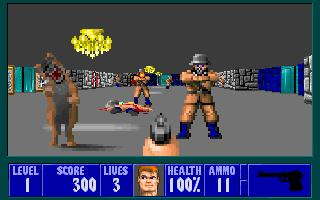
\includegraphics[width=\columnwidth]{wolfenstein.jpg}
        \caption{Kratek opis slike.} \label{fig:slika}
    \end{center}
\end{figure}

Pri pisanju poročila vključujte tudi reference na vire s katerimi ste si pomagali pri izdelavi seminarja. To so lahko pisni viri v obliki knjig \cite{Foley1994}, člankov \cite{Meng2015} ali drugih virov, ki jih dodajte med reference, spletne vire pa navajajte v nogi\footnote{\url{https://en.wikipedia.org/wiki/Computer_graphics}}.

Pri izdelavi igre se omejite na izdelavo enega samega nivoja igre, ki pa ga dodelajte in izpilite kolikor vam do\-pu\-šča predviden čas.

% do sem gre ven



\section{Pregled igre}
Naša igra je tretjeosebna pustolovščina, v kateri igraš pirata, ki želi svoj zaklad prinesti v pristanišče, brez da bi mu ga drugi pirati ukradli ali potopili ladjo. Igra je lahke do srednje težavnosti, namenjena širši množici. V zaprtem svetu, oblikovanem kot labirint, se glavni igralec izogiba drugim ladjam ali pa jih napada s svojim orožjem medtem ko išče pristanišče.

\subsection{Opis sveta}
Na tem mestu podajte grob opis sveta v igri, ki ga podrobenje definirate v sledečih podpoglavjih. Prav tako definirajte v kakšnem stilu bo izdelan svet (npr. realističen, stiliziran, risankast, ipd.). Opredelite tudi ali se bodo osebki v svetu pomikali v eni, dveh ali treh dimenzijah.

\subsubsection{Pregled}
Podpoglavje naj vsebuje podrobnejšo predstavitev sveta, s katerim interaktira uporabnik.

...

\subsubsection{Ozadje}
Opišite kako je predstavljeno ozadje sveta v igri - predeli s katerimi uporabnik ne interaktira a še vedno predstavljajo del sveta v igri (npr. nebo v ozadju, oddaljeni predmeti ipd.)

Nebo v ozadju bo predvidoma prikazano s Skyboxom, ...

\subsubsection{Ključne lokacije}
Izpostavite ključne lokacije v svetu, ki igrajo pomembno vlogo za uporabnika. Navedite zakaj so pomembne, na kakšne način bodo predstavljene (npr. domači tabor, nasprotnikov tabor, nahajališča dobrin  ipd.).

V svetu so najbolj ključna lokacija pristanišča, kjer igralec išče ciljno pristanišče - tam lahko ladjo popravi in nadgrajuje, shrani zaklad in dobi novo ciljno pristanišče. Druge pomembne lokacije so nahajališča dobrin, kjer lahko igralec pobere dodaten zaklad ali pa si popravi ladjo, ter druga pristanišča, kamor se igralec lahko vrne s delom preostalega zakladom, če mu nasprotniki uničejo ladjo, kamor pa ne more shraniti zaklada.

\subsubsection{Velikost}
Dobro opredelite velikost sveta in nivo na katerem bo s svetom interaktiral uporabnik. Kakšen pogled v svet bo primarno zajet v igri (npr. območje mize, sobe, mesta, pokrajine, kontineta, planeta, osončja, ozvezdja, galaksije ipd.)

Svet je velikosti neke pokrajine in je sestavljen iz kopna in morja. Igralec z ladjo pluje po morju, kopno pa je ovira in omejuje njegovo gibanje. Svet je velik, a vendar omejen. Igralec bo postavljen na naključno lokacijo v svetu, prebiti pa se mora do pravega pristanišča. 

\subsubsection{Objekti}
Predstavite poglavitne objekte, ki bodo zajeti v igri. Kje ste jih oz. jih boste pridobili. Ali ste jih oz. jih boste izdelali sami ipd.

Poglavitni objekti, ki bodo zajeti v igri, bodo ladje - igralčeva in nasprotnikove, pokrajina, sestavljena iz prednarejenih kosov in ključne lokacije, kot na primer pristanišče, ki jih bo izdelal naš grafični oblikovalec.

\subsubsection{Čas}
Opredelite hitrost časa v vaši igri. Kako hitro bodo minevala določena obdobja (npr. 1 dan v igri je 5 minut igralnega časa ali 1 minuta v igri predstavlja 1 uro igralnega časa).

Igralec ladjo premika v realnem času, premikanje ladje pa je pospešeno v primerjavi z realnim časom zaradi povečane odzivnosti. Ker igra ni razdeljena na obdobja, čas v igri nima igralnega pomena.

\subsection{Igralni pogon in uporabljene tehnologije}
V poglavju podrobno predstavite katere tehnologije ste uporabili pri izdelavi vašega seminarja. V kolikor ste uporabili kakšno dodatno ogrodje oz. orodje ga na tem mestu predstavite in pojasnite čemu.

Pri izdelavi našega seminarja bomo v prvem delu predvidoma uporabili WebGL, Three.js, Bullet.js ipd., v drugem delu pa se bomo obrnili na Unity.

\subsection{Pogled}
Definirajte kakšen bo pogled v vašo igro. Kakšno kamero boste uporabili, kaj vse bo uporabnik videl, kako boste poudarjali posamezne stvari ipd.

Pogled v našo igro bo omogočen na dva načina, med katerimi bo mogoče prosto menjati:
\begin{enumerate}
\item Pogled izza ladje - kamera bo vezana na zadnji del ladje in bo lokacijo in smer/rotacijo spreminjala skupaj z ladjo
\item Pogled od zgoraj - kamera bo na ladjo gledala od zgoraj navzdol, z nagibom in bo na ladjo vezana le z lokacijo, smer bo statična, rotacijo pa bo lahko nadzoroval uporabnik
\end{enumerate}

\small
\bibliographystyle{plain}
\bibliography{references}

\end{document}
